\chapter{Evaluation}

In this chapter we will describe a set of benchmarks, which will test our model
and enable us to compare it to other models. First we will describe the tasks
--- datasets and corresponding evaluation metrics, then we will talk about the
models. Results of the benchmarks are discussed in
Chapter~\ref{chapter:results}.

\section{Tasks}

Each task aims to test a different aspect of a model. Our aim was to design a
set of tasks, which can capture a model's capability to embed whole documents.
The major obstacle we faced was the lack of labeled datasets with longer pieces
of text (more than 512 tokens).

TODO: how did we solve the issue

TODO: complete list of task types

\subsubsection{Classification}

Classification tasks test model's capability to separate inputs based on a
complex feature. In our settings, classification tasks can tell us what
information the document embedding contains.


\subsection{IMDB Sentiment Analysis}

IMDB sentiment analysis task is a simple binary classification task. The dataset
contains movie reviews from the Internet Movie
Database\footnote{\url{www.imdb.com}} labaled as either positive or negative.
The dataset is commonly referred to as IMDB classification or sentiment
dataset~\cite{maas11}.

The dataset is split evenly to test and train set, each having 25000 reviews.
The dataset also contains 50000 unlabeled reviews. The label distribution in
both sets is uniform, each of of the two labels is represented by 12500 reviews.

As can be seen from the figure Figure~\ref{fig:imdb_word_token_dist} the reviews
are quite short with only 13.56\% being longer than 512 RoBERTa tokens.

\begin{figure}[ht]
  \centering
  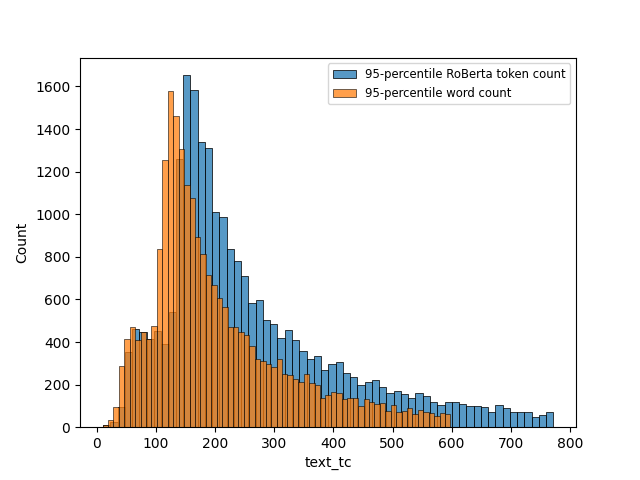
\includegraphics[width=0.9\textwidth]{img/imdb_word_token_distributions.png}
  \caption{Word count and token count distribution of 95-percentiles of
  reviews. The tokens are generated using RoBERTa's pretrained tokenizer from
  HuggingFace}\label{fig:imdb_word_token_dist}
\end{figure}

We included this task to see how our model compares in realtively undemanding
settings, while also evaluating its performence on shorter documents.

